\subsection*{Task 3}

\subsubsection*{a), b) and c)}

\begin{figure}[h!]
  \centering
  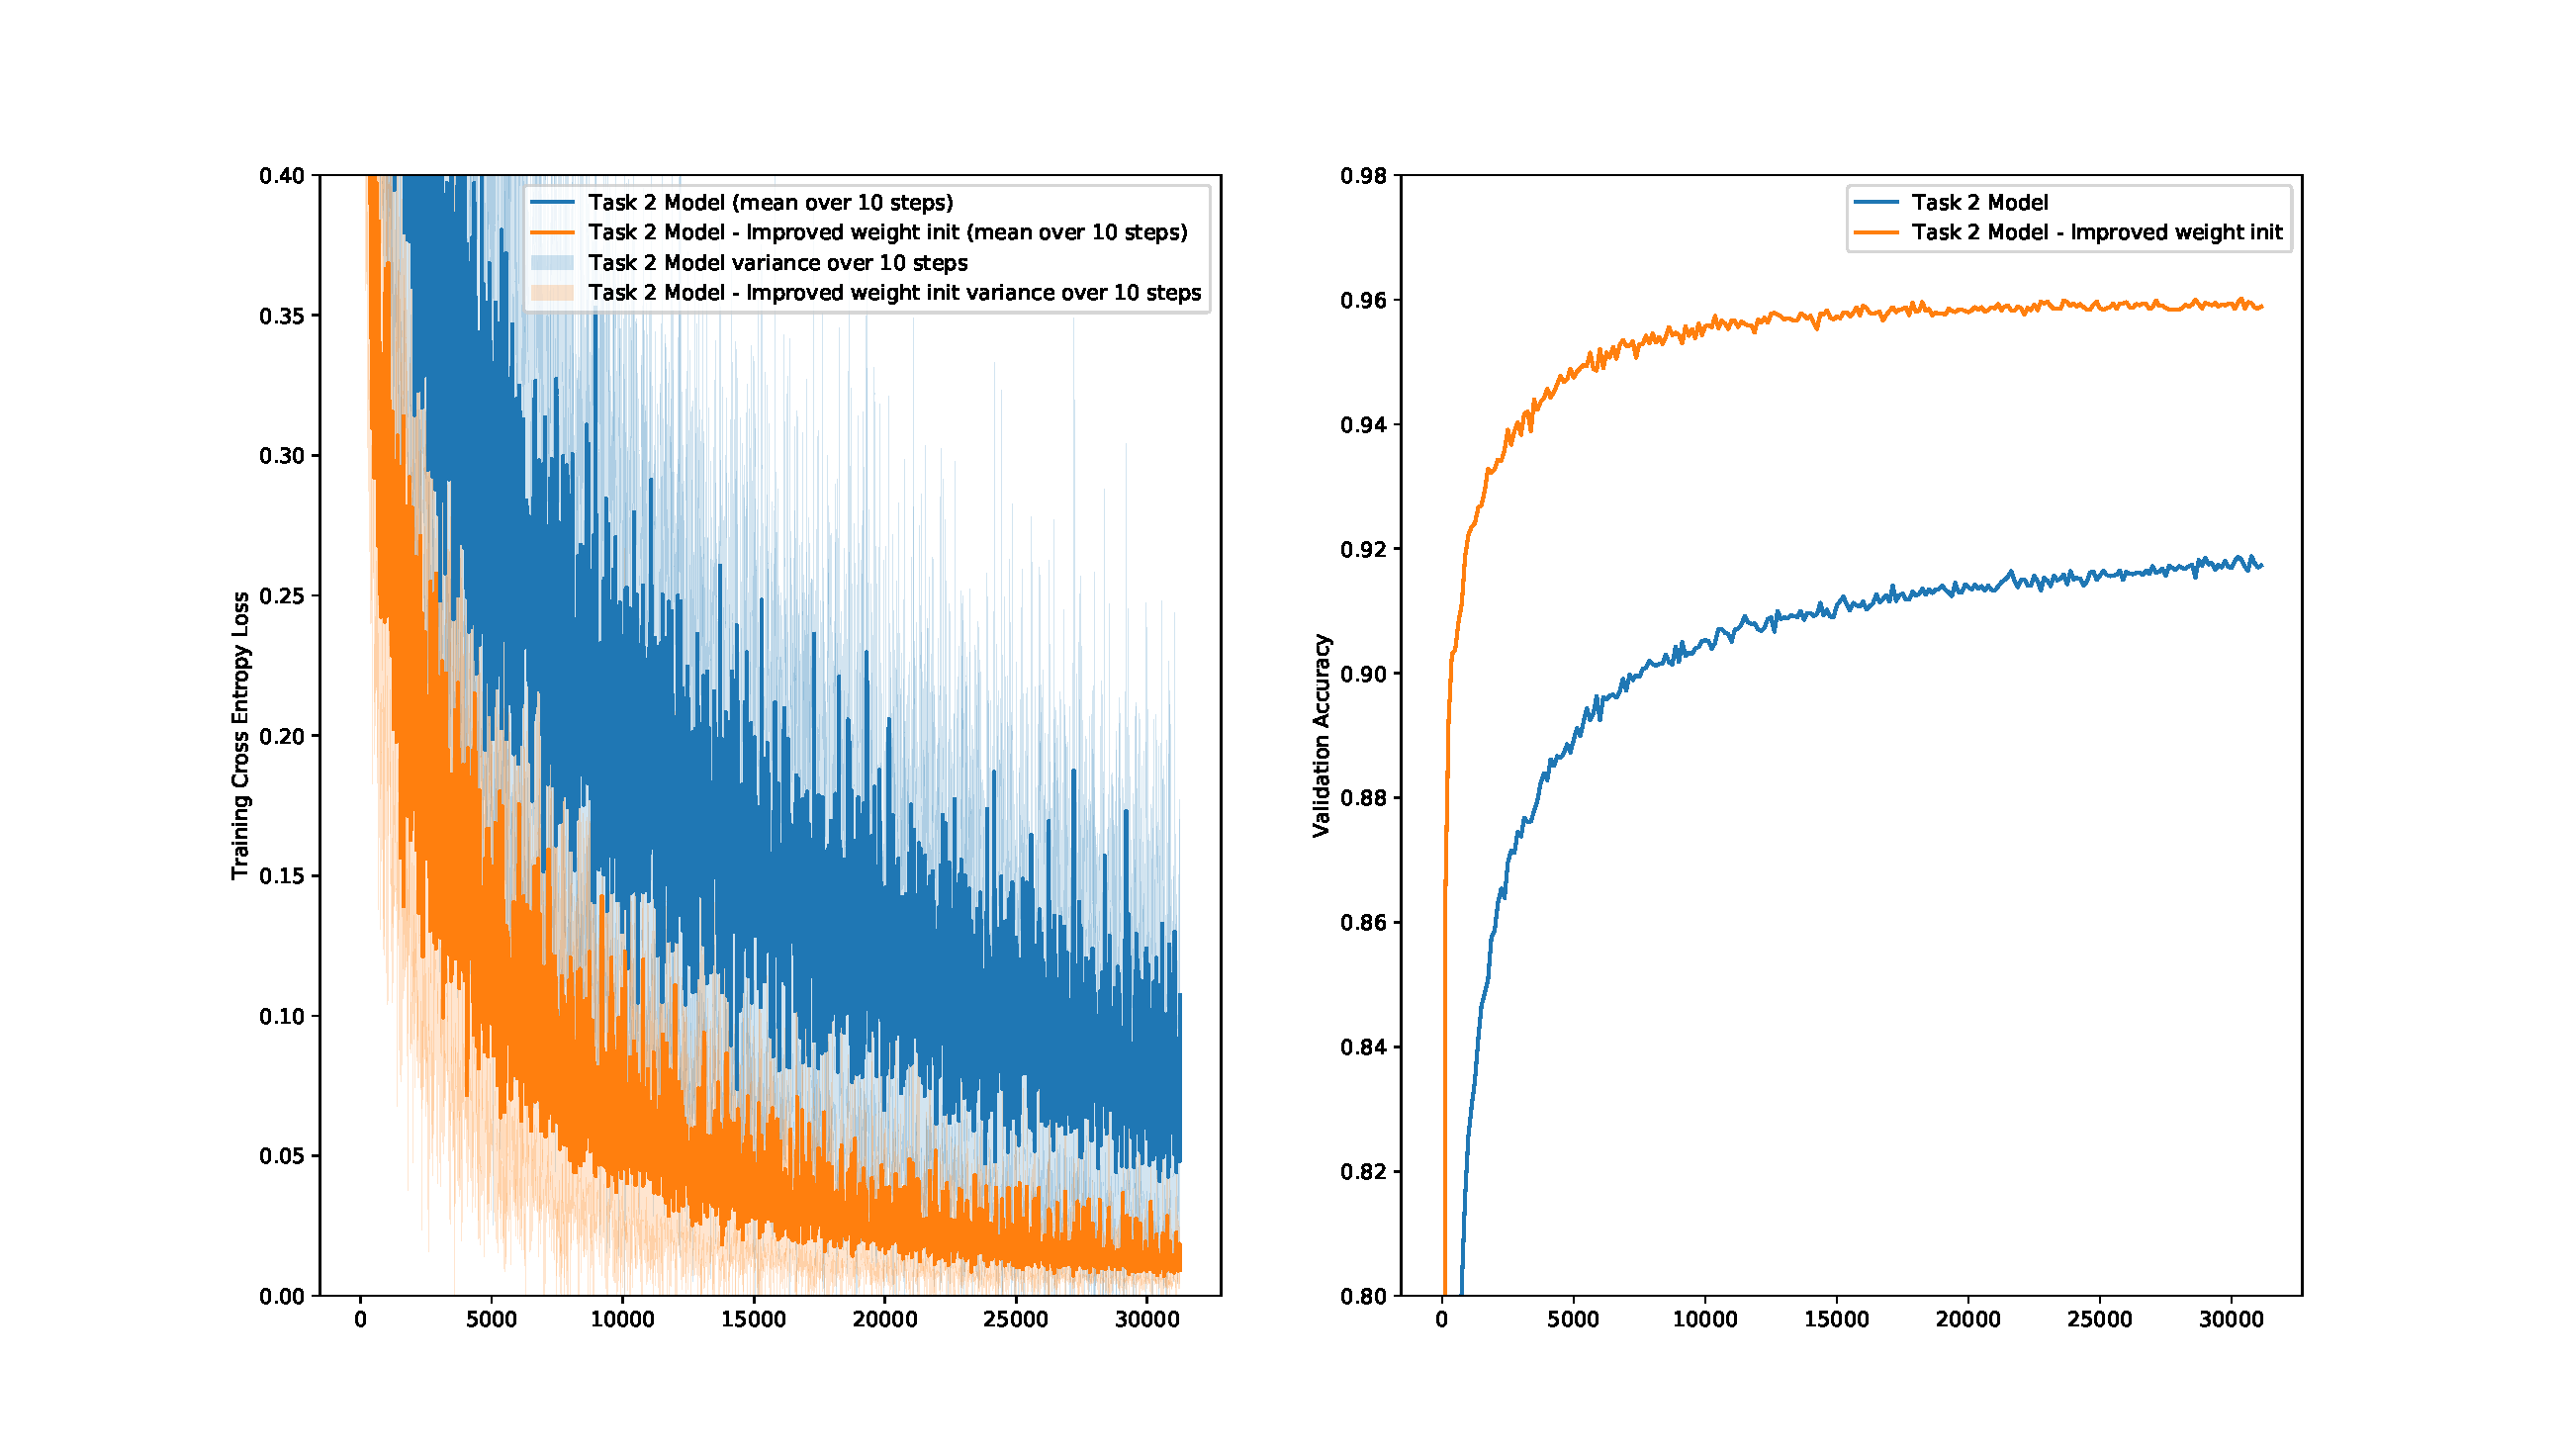
\includegraphics[clip, trim=3cm 0.5cm 3cm 0.5cm, width=\textwidth]{figures/Task3a.pdf}
  \caption{Training loss (left) and validation accuracy (right) with and without improved weight initialization.}
  \label{fig:task3:a}
\end{figure}

\begin{figure}[h!]
  \centering
  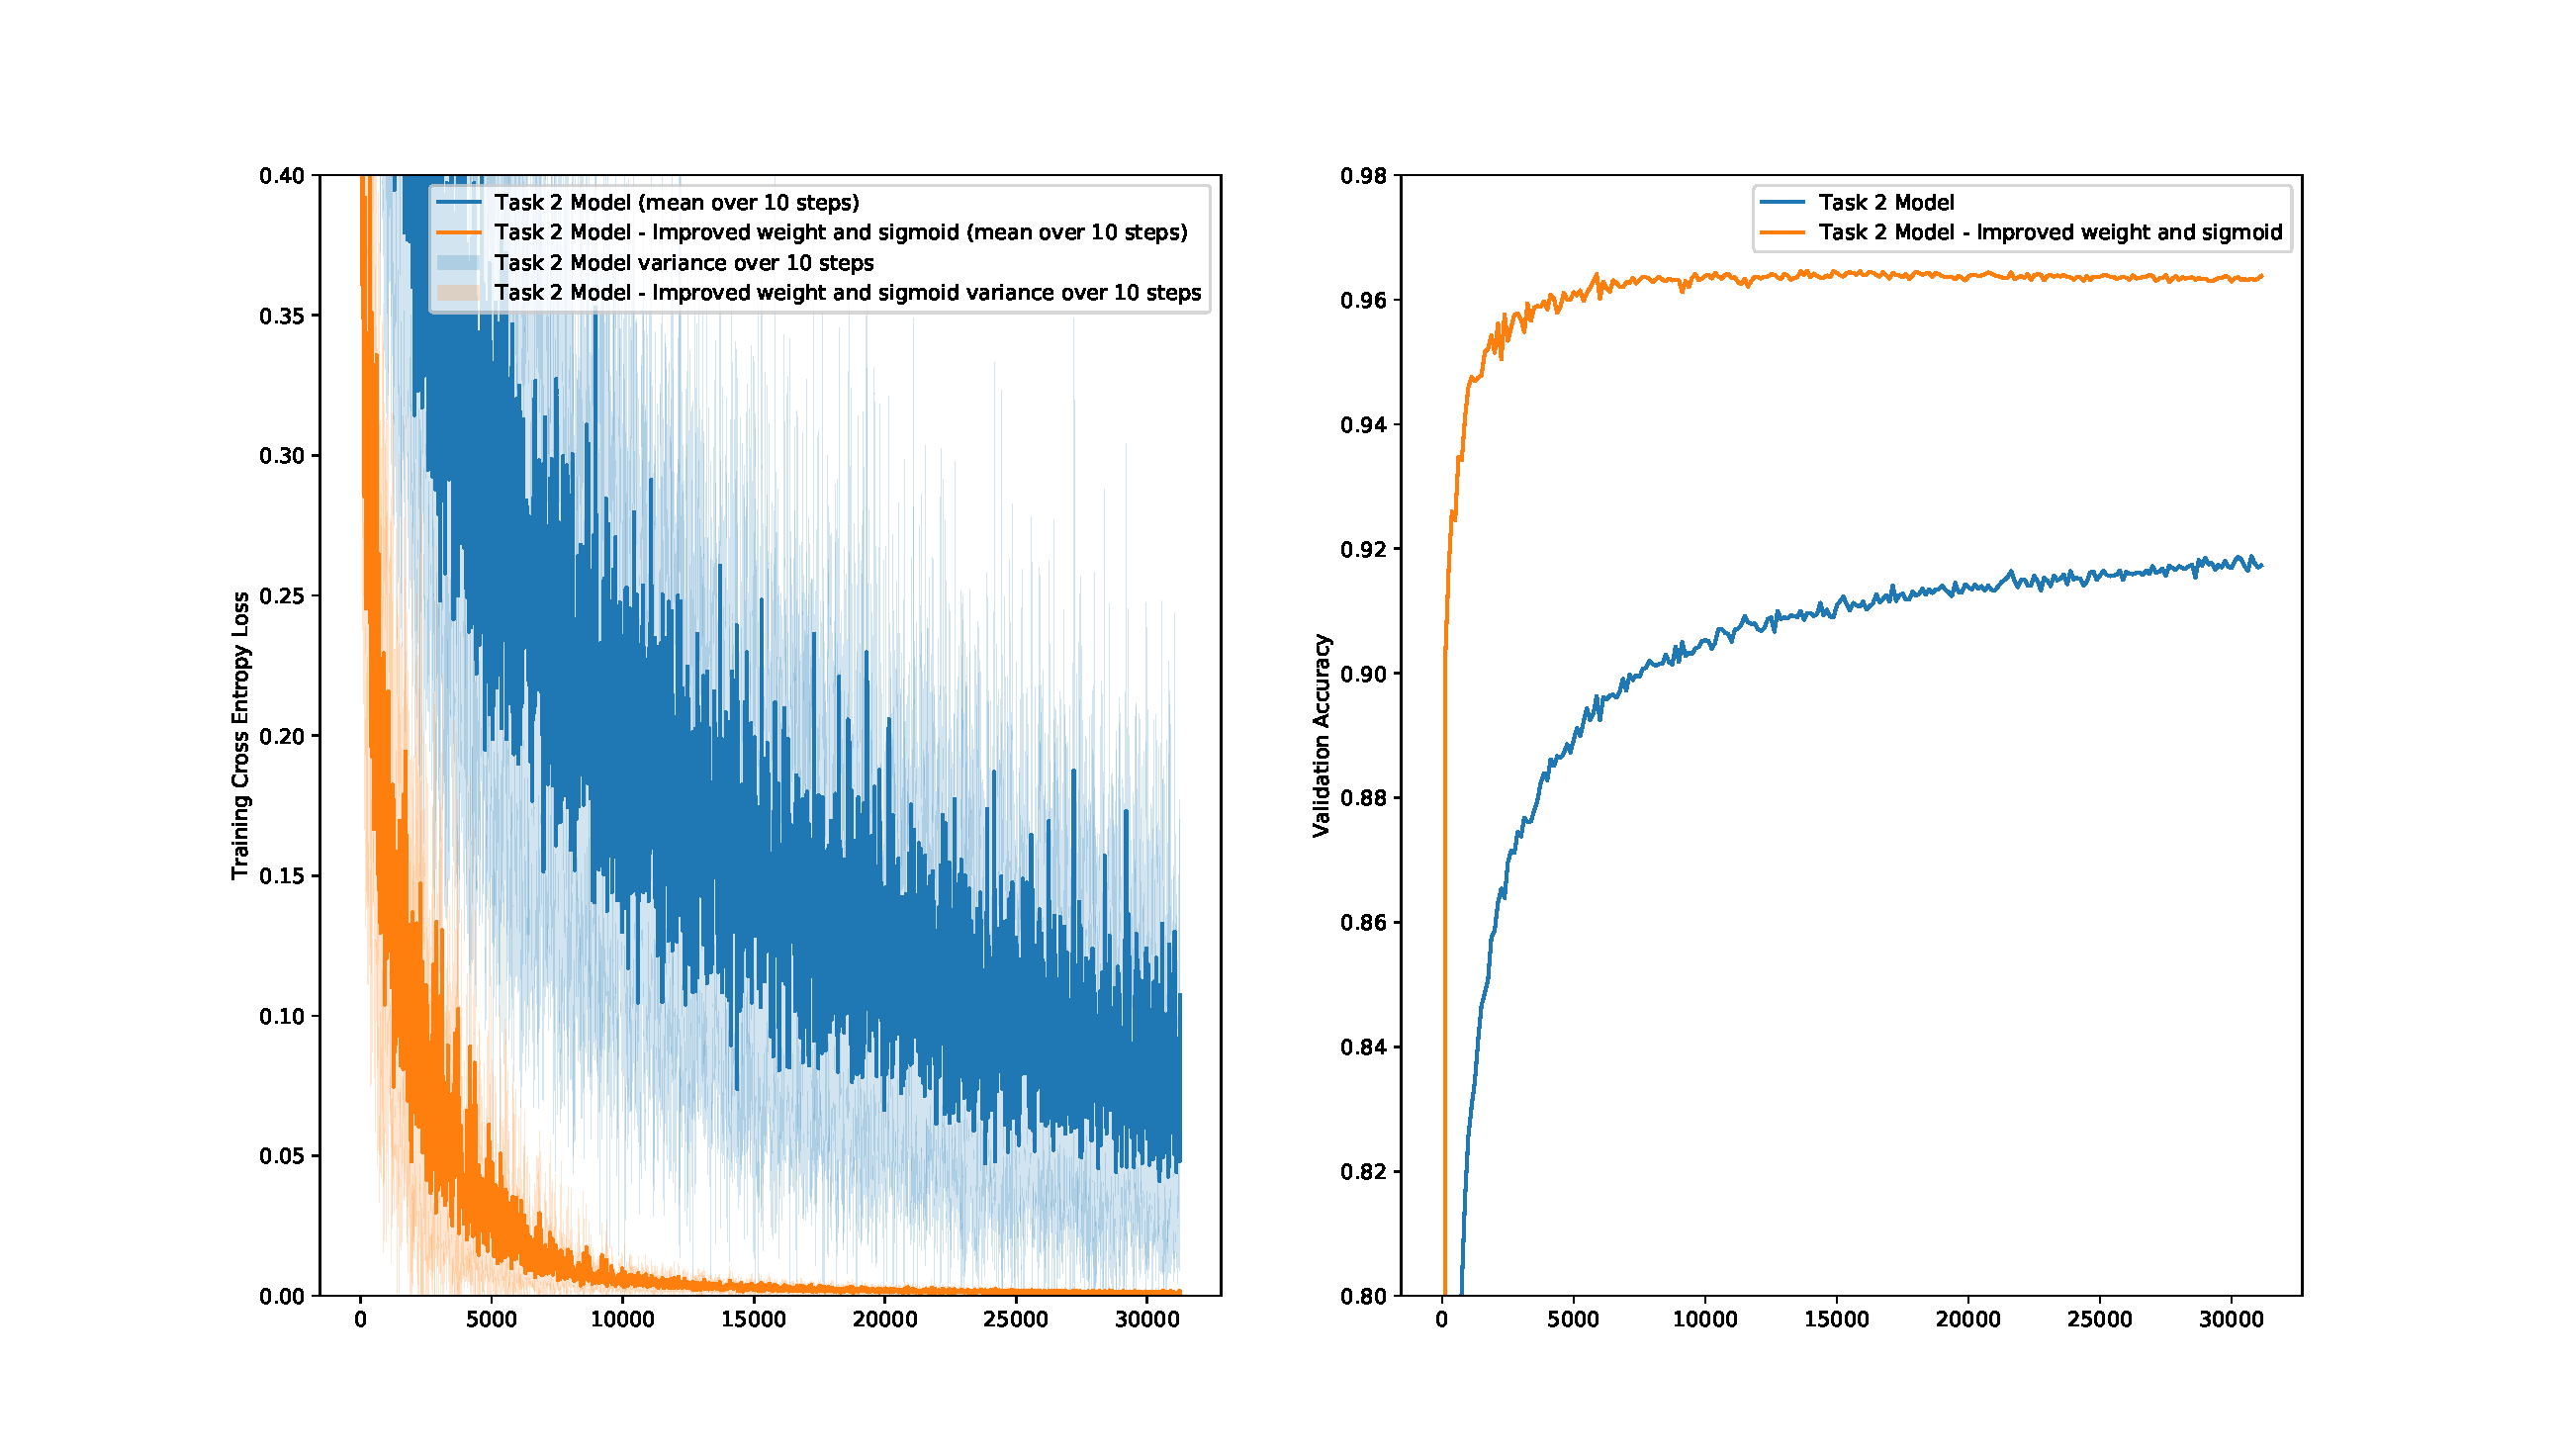
\includegraphics[clip, trim=3cm 0.5cm 3cm 0.5cm, width=\textwidth]{figures/Task3b.pdf}
  \caption{Training loss (left) and validation accuracy (right) with and without improved sigmoid and weight initialization.}
  \label{fig:task3:b}
\end{figure}

\begin{figure}[h!]
  \centering
  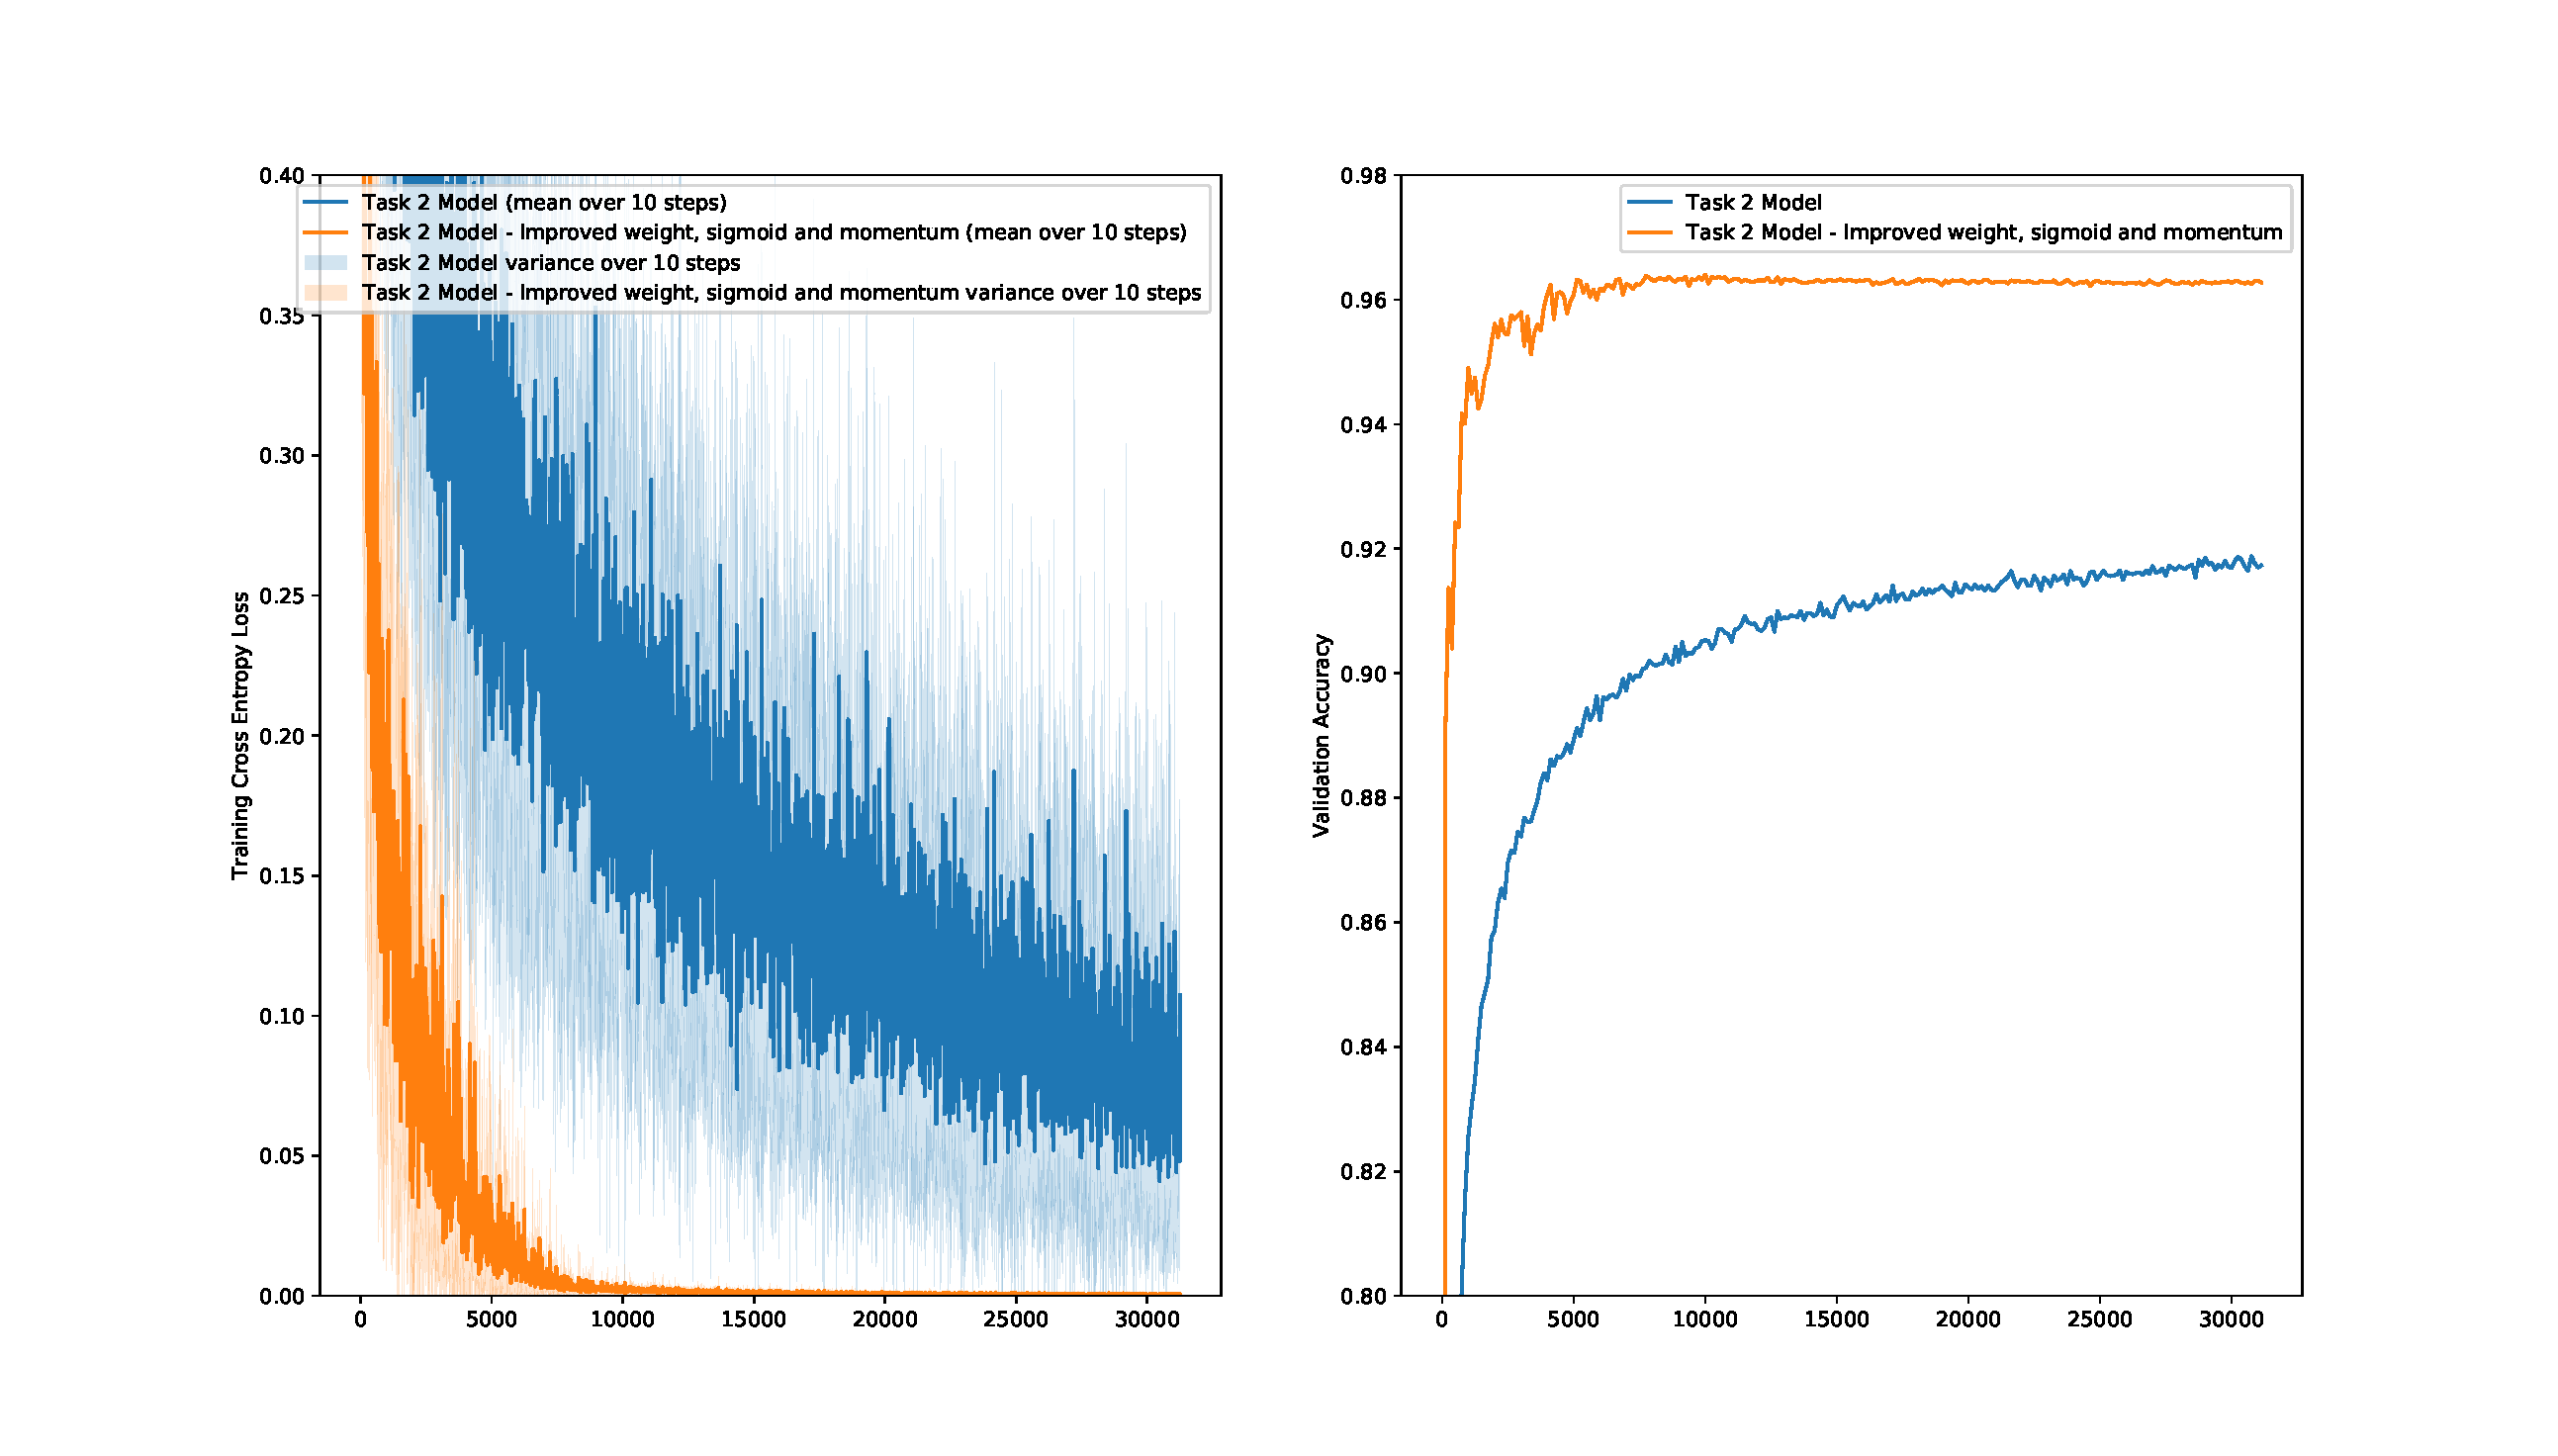
\includegraphics[clip, trim=3cm 1cm 3cm 1cm, width=\textwidth]{figures/Task3c.pdf}
  \caption{Training loss (left) and validation accuracy (right) with and without momentum, improved sigmoid and weight initialization.}
  \label{fig:task3:c}
\end{figure}

In \cref{fig:task3:a} we see an improvement in both convergence speed and accuracy by introducing an improved weight initialization. This is because the weights now are zero-centered, so the weight update can drive the individual weights in either direction. The sigmoid is however not zero-centered, meaning the input to the hidden layer will be biased in some direction, which again decreases the convergence speed.

By using the improved sigmoid, the convergence speed is much better, as seen in \cref{fig:task3:b}. The same argument as above applies, and since the output of each layer now is zero-centered, the weight update for all layers will not be biased in any direction. The weight initialization together with the improved sigmoid also ensures that the variance is close to 1 over the layers, such that the sigmoid is active over a larger area. With too large weights the sigmoid will saturate, giving too small gradients, and with too small weights the sigmoid will only be active in the linear area, so nonlinearities will not be modeled. This heavily affects the convergence speed, which again affects the accuracy when we use a maximum number of iterations as termination criteria.

Momentum is finally added in \cref{fig:task3:c}, but is not seen to impact the convergence speed or accuracy to any large extent. A slight increase in convergence speed is seen from the training loss, but by further inspection we also find that the accuracy has slightly decreased. This is probably just that the gradient descent has converged to a differnet minima due to the momentum, but it is insignificant in terms of overall performance.

As the training loss approaches zero when adding these tricks, one should be aware of possible overfitting. From \cref{fig:task2:loss_accuracy} we see clear signs of overfitting, as the training loss and accuracy is much better than for the validation set. The tricks we have implemented do not increase generalization in any way, so the problem of overfitting remains for the network in Task 3.
